\section{Pre-training}\label{sec:pretrain}

In this section, we will present two key components of pre-training: data and recipe, separately.

\subsection{Pre-training Data}
During the preparation of the pre-training data for Ling 2.0 models, we primarily focus on building an efficient data processing infrastructure and curating corpus that broadly covers high-quality universal data including but not limited general knowledge, code, math, multilingual content \emph{etc.}

\subsubsection{General Knowledge Data}

{\bfseries Data Cleaning from Raw Sources.}
LLMs gain general knowledge from large, diverse datasets like web pages, books, papers, and Wikipedia~\citep{soldaini2024dolmaopencorpustrillion}, which often suffer quality issues. We created specialized cleaning pipelines combining rules and models tailored per data type. For web data, we extract content using the trafilatura parser\footnote{\url{https://trafilatura.readthedocs.io/en/latest/}} and apply sampling-based checks to identify common low-quality patterns. Targeted cleaning removes ads, embedded URLs, symbol-heavy texts, fixes Markdown and table parsing. HTML/PDF parsers are continuously improved to enhance extraction accuracy.

{\bfseries Detection and Remediation of New Low-Quality Data.} 
Iterative sampling reveals new low-quality data, addressed with an automated detection and rule-generation pipeline involving: 1) Multi-channel Recall: Using classifiers, lightweight LLM scoring, and perplexity (PPL) to flag suspect samples; 2) Issue Analysis: LLMs categorize issues as known or new rule cases; 3) Rule Generation: LLMs create cleaning rules based on issue context and a quality-issue database; 4) Rule Generalization: Grouping similar cases for LLM-driven abstraction to broaden rule applicability. New rules undergo human review before integration, speeding detection and remediation.

{\bfseries High-Quality Filtering and Knowledge Text Rewriting.} 
Despite cleaning, datasets remain massive. To improve training, we develop  
High-Quality Filtering pipeline. Inspired by FineWeb-Edu~\citep{penedo2024finewebdatasetsdecantingweb}, we train feature models by data type (e.g., Chinese/English web, books, papers) to assess quality, education level, knowledge density, and domain. Iterative experiments identify optimal subsets; for instance, our English web subset is ~5× larger than FineWeb-Edu and outperforms it on knowledge benchmarks. Models struggle with complex or rare knowledge in raw text. We use recall-rewrite: (i) select candidate texts by knowledge density, STEM domain, and QA features; (ii) apply semi-synthetic rewriting like Wikipedia-style structure, QA conversion, and concise summaries. Ablation experiments show consistent gains on MMLU~\citep{mmlu}, CMMLU~\citep{cmmlu}, and CEval~\citep{ceval} benchmarks.







\subsubsection{Reasoning Data}
We aim to endow Ling 2.0 with powerful general reasoning capabilities, which primarily encompass programming and mathematical skills. To this end, we optimize our reasoning data from multiple perspectives, including scale, diversity, and quality.

\subsubsubsection{Ling Code Corpus}
To support the training of high-performance coding-oriented LLMs, we constructed a diverse, large-scale, and quality-stratified \emph{Ling Code Corpus} that integrates multiple data sources, covering source code, code-related natural language data, and synthetic instructional data. 
Our curation pipeline emphasizes both breadth of programming language and domain coverage, and the depth of quality control.
\label{1b-coder-section}

We collected raw source code from Github repositories. We use
multilingual fine-grained cleaning rules tailored to the syntax and conventions of each language. We apply Lint-based\footnote{\url{https://en.wikipedia.org/wiki/Lint_(software)}} syntactic validation to remove files with compilation or structural errors. This yields our source code corpus covering 660 programming languages. We further conduct 1) quality stratification according to code style/readability, norm adherence, and complexity/difficulty; 2) code rephrasing and paraphrasing techniques, to generate additional high quality augmented code data. In addition to github repositories, we 1) reconstructed commit data from GHArchive\footnote{\url{https://www.gharchive.org/}} by replaying event sequences (e.g., pull requests, issues, merges) at the repository level; 2) iteratively optimize our code-oriented html-parsers and cleaning operators to curate code-related pages, tutorials, developers' discussions from Common Crawl and Web; 3) curated a large collection of programming-competition data consist of problem statements from diverse platforms, user submissions, and related user discussions and commentary threads. 

{\bfseries Evaluating the Ling Code Corpus. }
We designed a lightweight verification strategy, i.e., training small-sized coding models (e.g., 1B size) from scratch to measure the performance of our code data. Experiments show that from-scratch training on single-type code data provides a reliable proxy for full-scale performance. This finding enables efficient early-stage validation of architecture and training recipes before scaling to tens or hundreds of billions of parameters. We show our results on 1B models (Ling-coder-1B) compared with Qwen2.5-Coder-1.5B-Base~\citep{hui2024qwen2} and Qwen3-1.7B-Base~\citep{qwen3} in Figure~\ref{fig:coder-1b-main-avg}. The results are promising that we have equivalent or even better results on mainstream benchmarks compared with Qwen2.5-Coder-1.5B-Base. This is achieved by consuming only 2T tokens of our code data from scratch, with an additional 300B anealing phase. More details can be found in Appendix \ref{appendix:coder}







\begin{figure}[t!]
    \centering
    \begin{subfigure}[b]{0.32\textwidth}
        \centering
        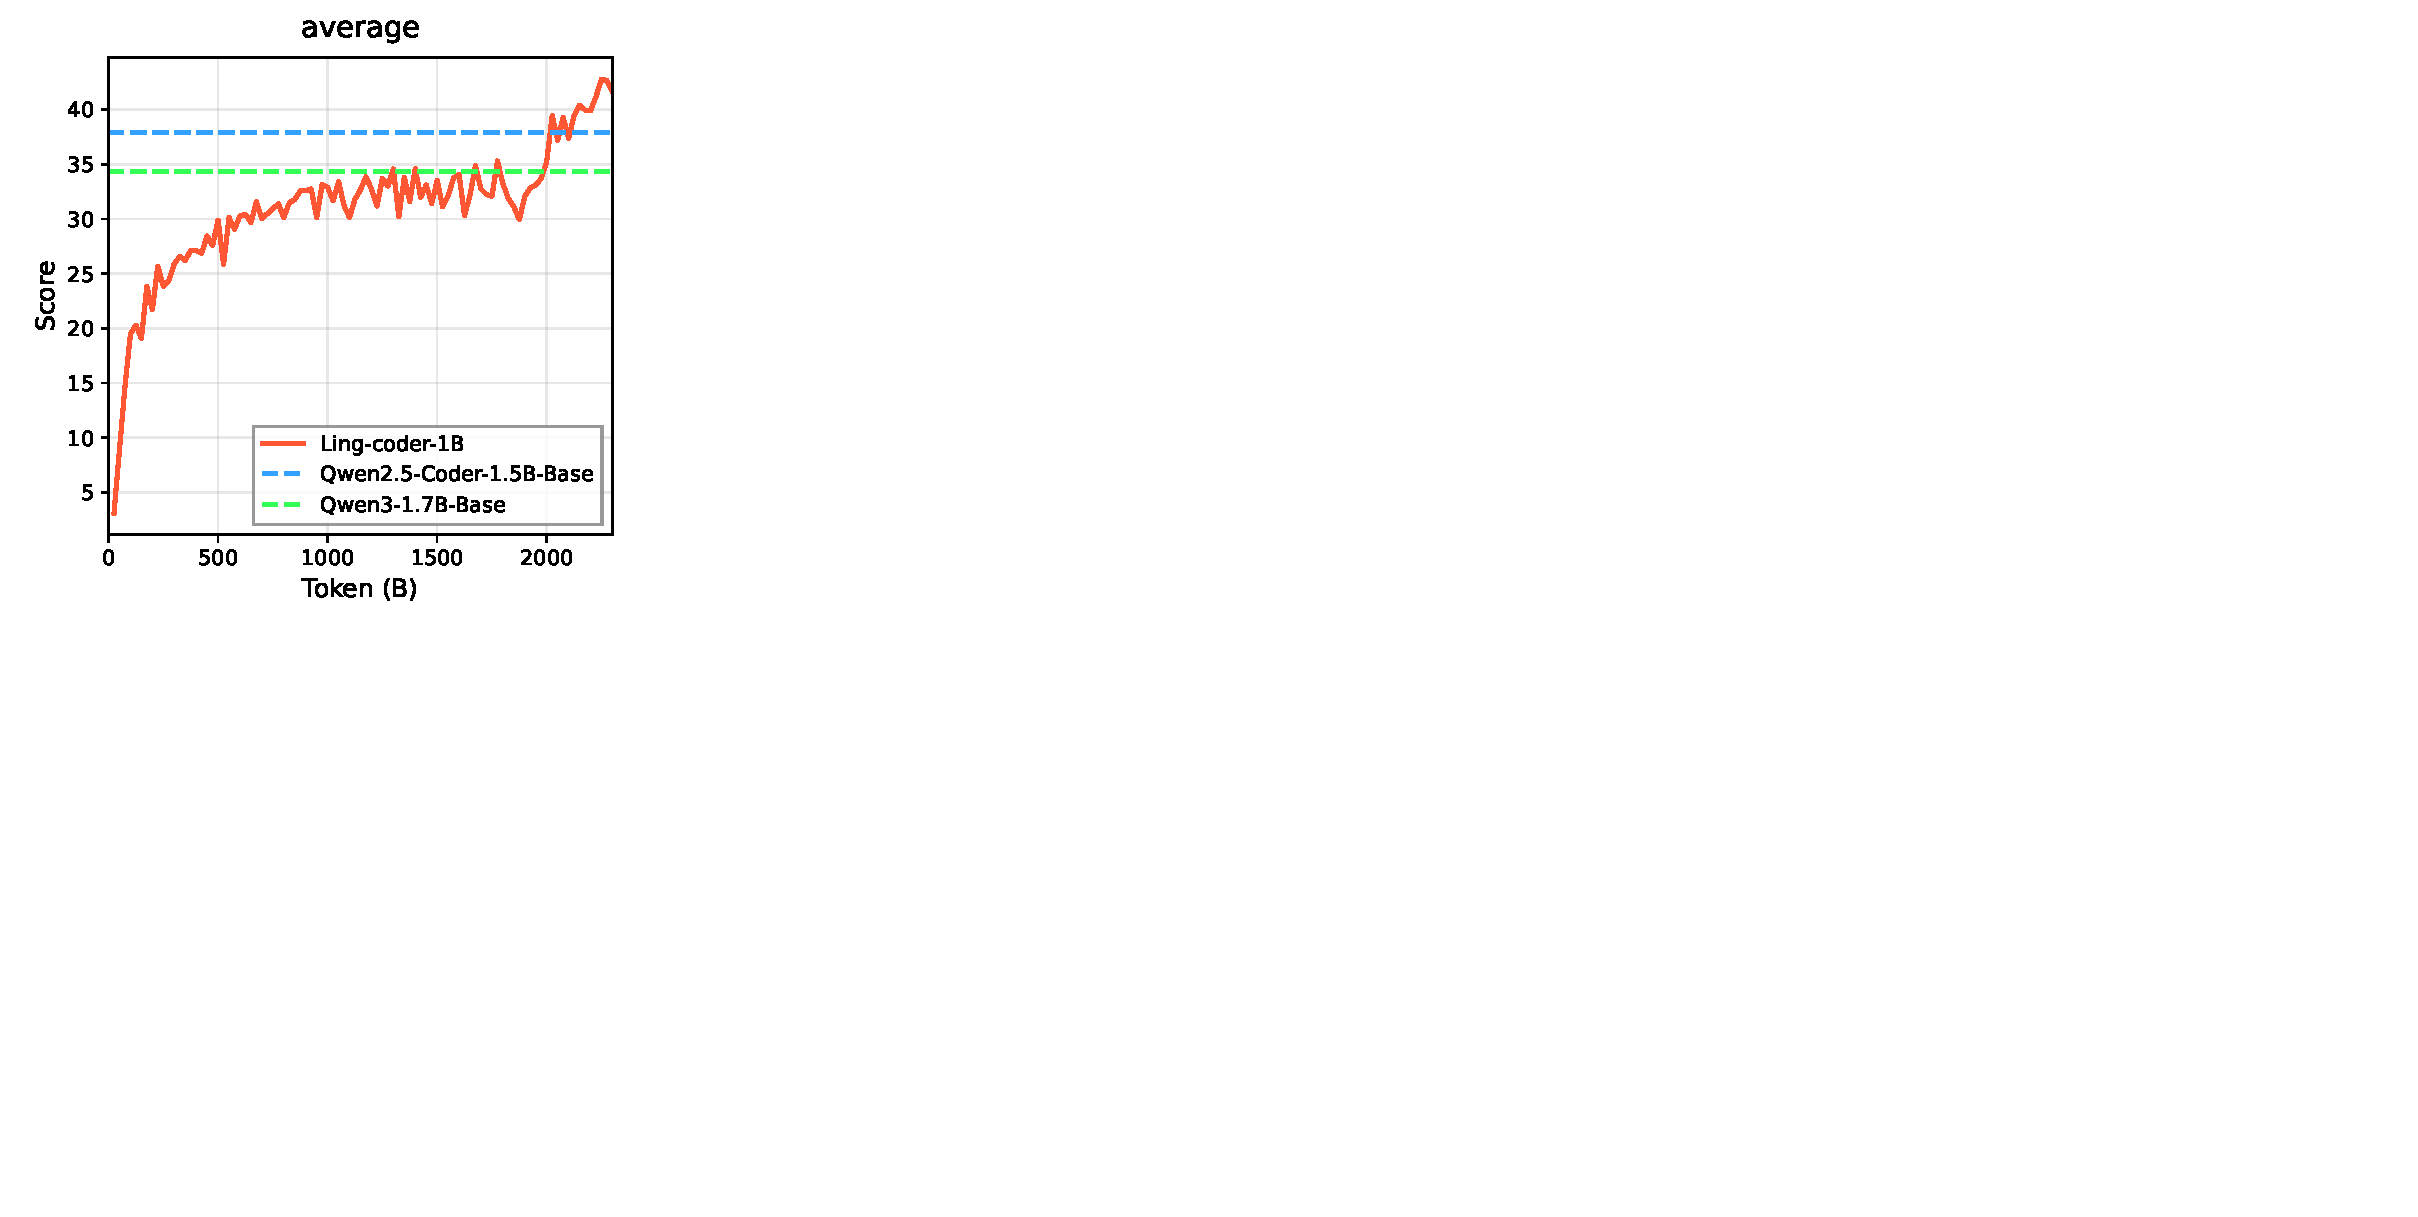
\includegraphics[width=0.9\textwidth]{figs/ling_math_coder_avg.pdf}
        \caption{Overall performance of Ling Code Corpus on 1B models.}
        \label{fig:coder-1b-main-avg}
    \end{subfigure}
    \hfill 
    \begin{subfigure}[b]{0.315\textwidth} 
        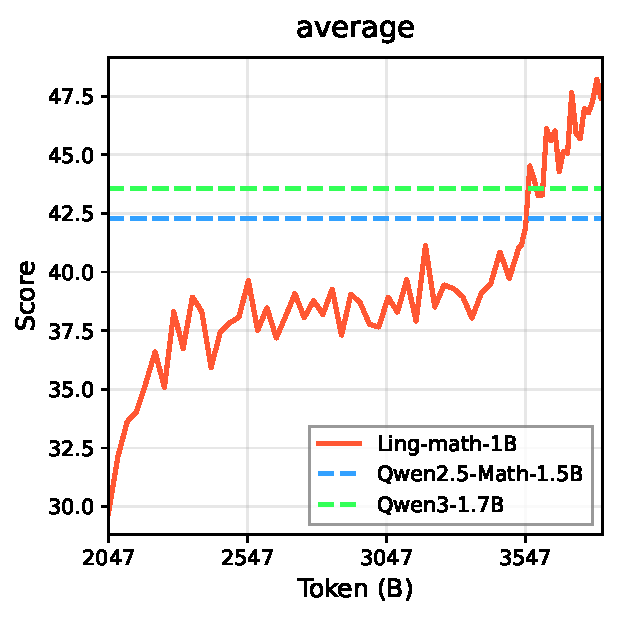
\includegraphics[width=0.93\textwidth]{figs/ling_math_1b_fig_avg.pdf}
        \caption{Overall performance of Ling Math Corpus on 1B models.}
        \label{fig:math:a}
    \end{subfigure}
    \hfill 
    \begin{subfigure}[b]{0.35\textwidth} 
        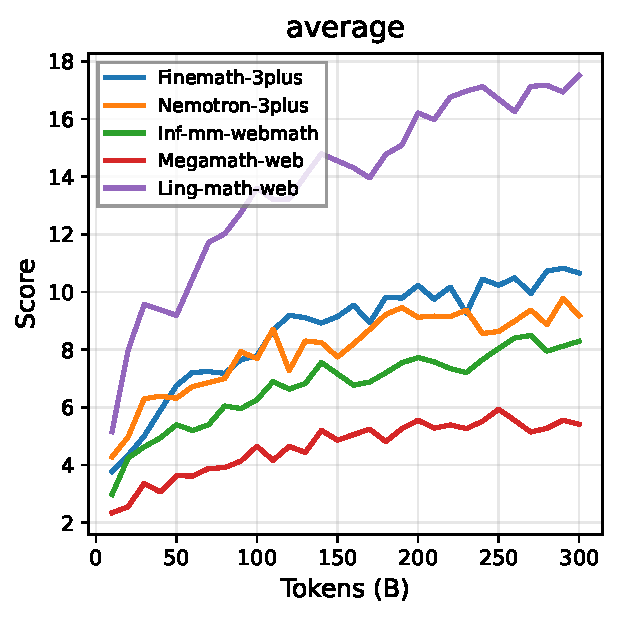
\includegraphics[width=0.83\textwidth]{figs/math_all_metrics_avg.pdf}
        \caption{Comparison of Ling Math Corpus with open-source mathematical web data.}
        \label{fig:math:b}
    \end{subfigure}
    \caption{Performance of Ling Code Corpus (a) and Ling Math Corpus (b, c).}
    \label{fig:scaling}
\end{figure}









\subsubsubsection{Ling Math Corpus}
To train Ling 2.0 models of varying scales, we assembled a mathematics corpus drawn from web pages, textbooks, research papers, code repositories, problem banks, and synthetic sources. A multi-stage processing pipeline—comprising parsing, recall, filtering, rewriting, and synthesis—was designed to curate this corpus.

We iteratively improved the PDF and HTML parser to ensure the completeness of mathematical content. We build fastText classifiers to recall math data from a huge candidate pool. We then fine-tune small language models to develop LLM-Filter and LLM-Refiner that can filter and refine data that contain mathematical knowledge or step-by-step problem solving process.
In addition, we employ synthetic data generation to create a diverse range of mathematical question-answer (Q\&A) pairs, varying in difficulty and incorporating step-by-step reasoning processes. This includes 1) Q\&A pairs extraction from web and book; 2) development of a sophisticated question generator for high quality and realistic mathematical problems; 3) the build of a large-scale mathematical concept graph~\citep{chen2025arrows} to extend the knowledge boundaries of our model.

{\bfseries Evaluating the Ling Math Corpus. }
To empirically validate the efficacy of our mathematical corpus, we use a continual-training then annealing strategy with only math corpus on a pre-trained Ling-coder-1B model introduced in Section \ref{1b-coder-section} for over 1.8T tokens, in which the last 300B is used for annealing training. Due to the space limit, we only present the performance results on the average value of benchmarks. As shown in Figure~\ref{fig:math:a}, the resulting Ling-math-1B model exhibited performance superior to the competitive Qwen2.5-Math-1.5B-Base~\citep{yang2024qwen25mathtechnicalreportmathematical} and Qwen3-1.7B-Base~\citep{qwen3} on mainstream mathematical benchmarks (e.g. GSM8K~\citep{gsm8k}, MATH~\citep{math}, CollegeMath~\citep{college-math}, OlympiadBench~\citep{olympiadbench}, CMATH~\citep{cmath}, MathBench~\citep{mathbench} \emph{etc.}). 

Furthermore, a specific comparative analysis was conducted to evaluate the contribution of our curated mathematical web data. Using the same 1B-model training paradigm, we benchmarked our proprietary web data against a suite of well-regarded open-source datasets, namely Infi-mm-math~\citep{han2024infimmwebmath40badvancingmultimodalpretraining}, finemath-3plus~\citep{allal2025smollm2smolgoesbig}, megamath~\citep{zhou2025megamath}, and nemotron-cc~\citep{mahabadi2025nemotron}. The Ling-math-web-1B model trained on our web data demonstrated a markedly superior performance shown in Figure~\ref{fig:math:b}. This finding validates the effectiveness of our specialized web data acquisition and refinement pipeline, a critical factor contributing to the high quality of our pre-training data (detailed in Appendix \ref{appendix:math}).


\subsubsection{Multilingual Data}

To enhance multilingual capabilities, we expand the tokenizer vocabulary from 128K in Ling 1.5 to 156K, with targeted additions of multilingual tokens. For multilingual corpus, we curate approximately 2TB of high-quality multilingual data from open web sources and parallel corpora. The data undergoes rigorous preprocessing, including language identification, filtering, cleaning, and deduplication, to ensure linguistic diversity and data integrity. The corpus spans a broad range of about 30 languages and diverse domains, including web text, code, mathematics, Wikipedia, and parallel sentence pairs, supporting robust cross-lingual understanding. Furthermore, multilingual data constitutes 4\% of the total pre-training data. Through experimentation, we determined an optimal distribution that significantly improves minor language performance while maintaining Chinese and English capabilities. Our findings indicate that data from Romance and Germanic languages have less negative impact on core languages, whereas data from certain other language families requires more careful balancing. More details can be found in Appendix \ref{sec:multilingual}.


\subsubsection{Long-Context Data} 
To build long-context ability we implement a \emph{retrieve–synthesize–validate} pipeline over heterogeneous sources (web pages, books/novels, scientific articles, software docs, etc.). Quality controls include: 
\begin{itemize}
    \item \emph{Linguistic hygiene}: Combination of rule checking and model recognition to identify and repair issues such as paragraph duplication, language mixing, and content truncation.
    \item \emph{Semantic consistency checks}: Using model-aided detection and a small amount of manual observation to detect logical contradictions within the text to filter data, and optimize relevant recall/synthesis logic.
    \item \emph{Long-range quality scoring}: We eliminate low-quality long text content using the \emph{PPL gap} between long- and short-window evaluations, combined with auxiliary scores. 
\end{itemize}
This pipeline yields \textasciitilde1.2\,\textsc{T} high-quality long-text tokens.


\subsubsection{Data Infrastructure}
Training large-scale language models presents major challenges in data infrastructure efficiency, scalability, and governance. To tackle issues like inefficient collaboration, opaque lineage, and slow iteration, we built a next-generation infrastructure based on two core principles: \emph{Data-as-Code} and a \emph{Unified Data Lakehouse}.

{\bfseries Data-as-Code: Automating CI/CD workflows.} 
We codify the entire data pipeline and manage it via version control (e.g., Git) to enable automated, reproducible workflows. This aligns with top ML platforms that standardize workflows through code-driven orchestration~\citep{datainfra1}. We developed a unified \emph{AIDataOps} library with 50+ data operators across modalities, integrated into an automated CI/CD system. Benefits include transparent, traceable end-to-end data lineage and fully automated feature development, cutting R\&D iteration cycles from months to days.

{\bfseries Unified Data Lakehouse and Wide-Table Architecture.}  
To overcome data silos from hundreds of scattered datasets, we implemented a unified lakehouse~\citep{datainfra2} with a wide logical table aggregating major domains like web pages and code. This central hub simplifies discovery and analysis, supports elastic scalability without full-table rebuilds, and achieves over 20 TB/hour I/O throughput, removing data processing bottlenecks for large-scale training.

Combining these principles, we created a powerful data engine essential for building the Ling 2.0 corpus. This enabled constructing a trillion-record web-wide table and processing 30 billion trainable data points in two days, accelerating model development and enabling complex future data exploration. More information can be found in Appendix \ref{appendix:data:infra}







\subsection{Pre-training Recipe}
Ling 2.0 pre-training adopts a multi-stage strategy with stage-tailored data mixes, and uses a WSM (warmup-stable-merge) scheduler~\citep{tian2025wsmdecayfreelearningrate} that replaces LR decay with checkpoint merging for greater flexibility and effectiveness. 
Next, we detail the training recipe of Ling 2.0. 

\subsubsection{Hyper-Parameters}

\paratitle{{Model Hyper-Parameters. }}
Based on a deep analysis of scaling laws in Section~\ref{sec:scaling4moe}, Ling 2.0 employs a high-sparsity, fine-grained MoE architecture. Each MoE layer comprises one shared and 256 routed experts, activating 8 experts per token. 
For stability, the first several layers are dense layers.
The attention head dimension is fixed at 128 across all model sizes.
We use Multi-Token Prediction (MTP) with depth 1.
All parameters are randomly initialized with standard deviation 0.006.
Other architectural parameters scale with model size; see Table~\ref{tab:model-specs} for details.

\paratitle{{Training Hyper-Parameters. }}
We use AdamW~\citep{adamw} with $\beta_1{=}0.9$, $\beta_2{=}0.95$, weight decay~$0.1$, and gradient-norm clipping~$1.0$.
Pre-training uses a 4K context window for the first 20T tokens, followed by 150B tokens with 32K contexts. We set the bias-update rate $\gamma{=}0.001$ for the auxiliary-loss-free load-balancing term and an MTP loss weight of $0.1$. After context extension, the bias-update rate is set to $0.0001$ for the rest of training.
Guided by the Ling scaling laws in Section~\ref{sec:scaling4parametres}, we determined the learning rate and batch size for Ling 2.0 and summarize them in Table~\ref{tab:model-specs}. 
For the batch size, we apply a batch-size ramp for the first $\approx\!500\mathrm{B}$ tokens (e.g., from 3{,}024 to the peak), then keep it in the remaining training. 
For the learning rate, we use the novel {WSM} (warmup-stable-merge) scheduler: linear warmup for the first 2{,}000 steps to a peak LR, then \emph{constant LR} until training ends; the final ``annealing'' is achieved by checkpoint merging instead of LR decay (see Section~\ref{sec:merging} for details). 


\subsubsection{Multi-Stage Training}
Ling 2.0 adopts a multi-stage pretraining strategy comprising: (1) general pre-training on a large-scale general corpus; and (2) mid-training on a medium-scale, task-specific corpus.



\begin{figure*}[t]
    \centering
    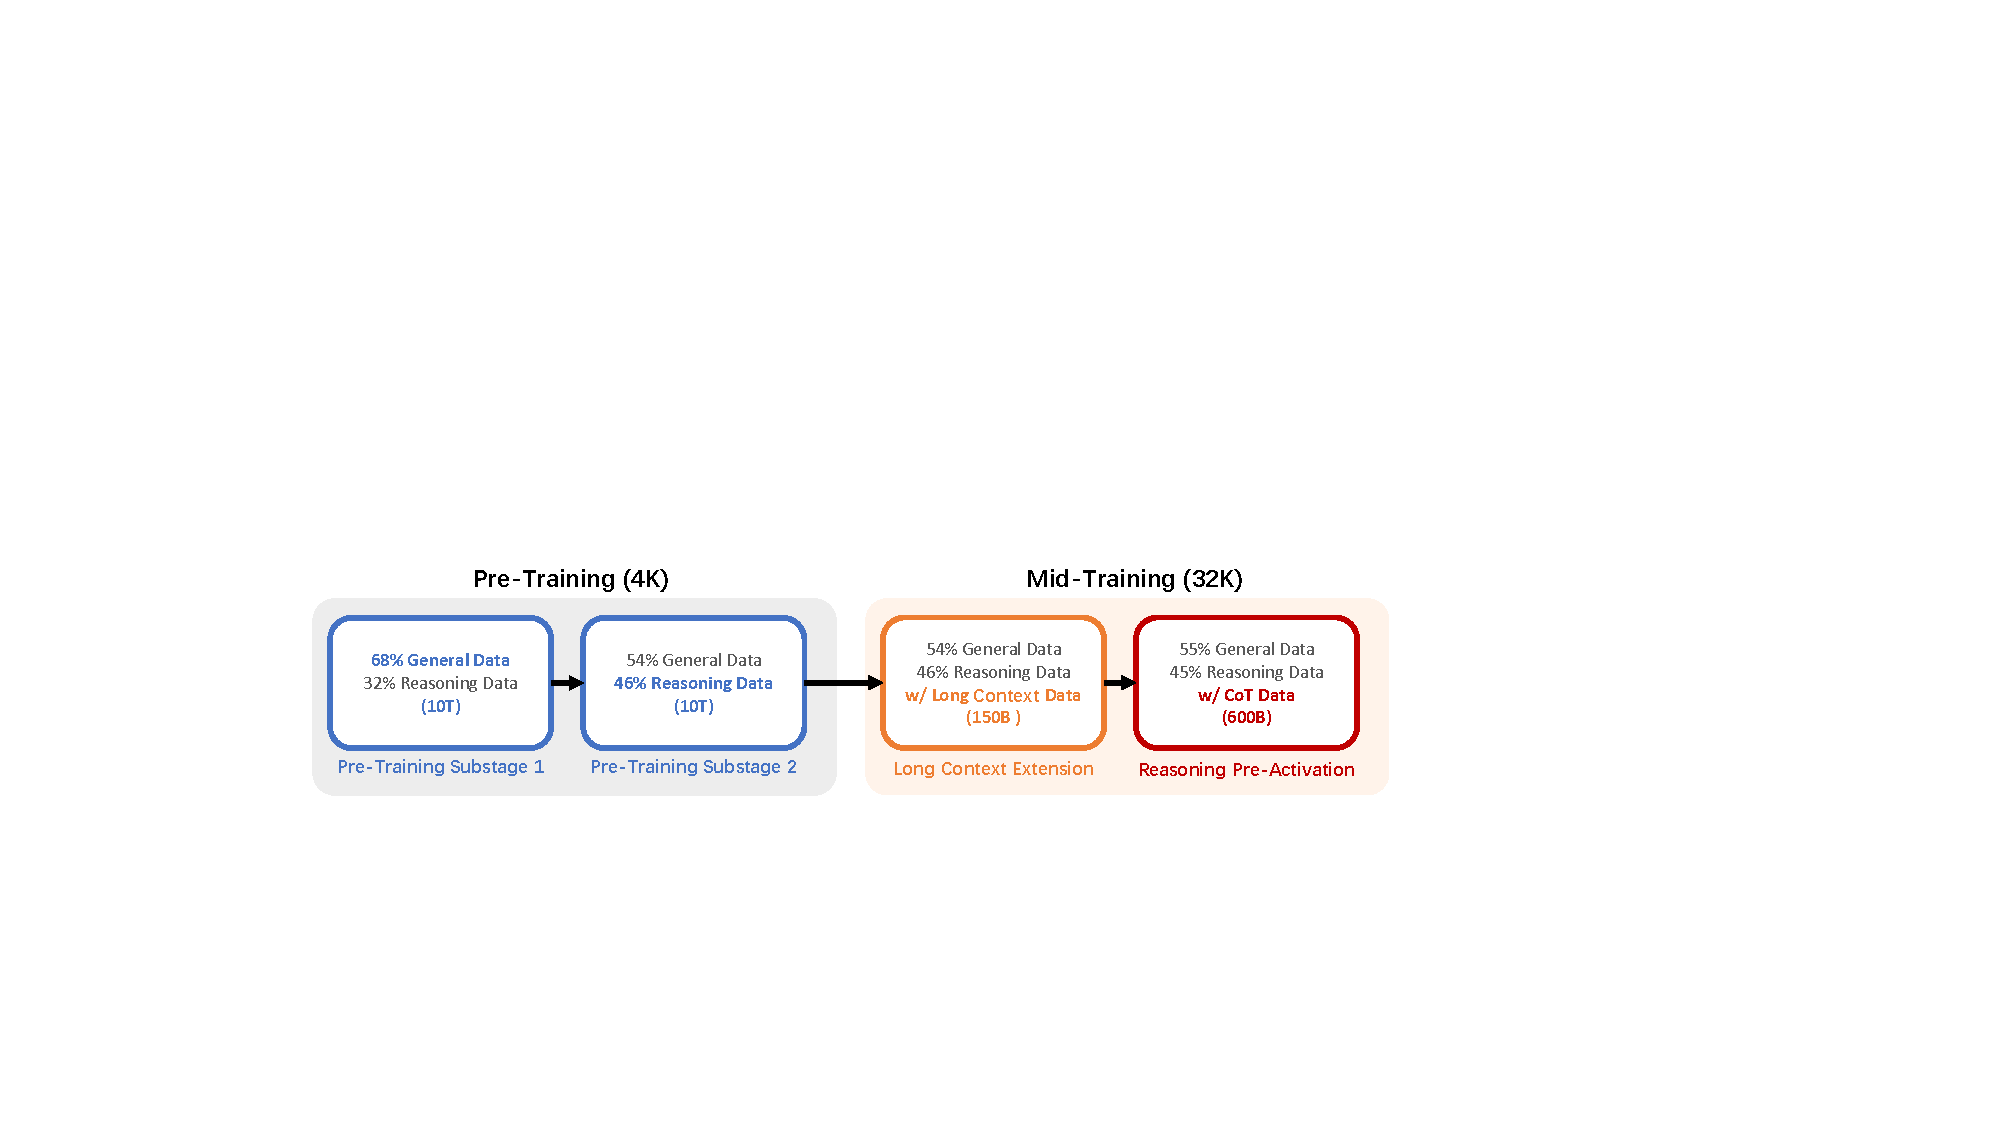
\includegraphics[width=0.95\textwidth]{figs/multi_stage.pdf}
    \caption{{Pre-training and mid-training stages of Ling 2.0.} We adopt a multi-stage training strategy that progressively expands the context window from 4K to 128K and introduces reasoning and CoT data in advance to pre-activate the model’s reasoning ability. }
    \label{fig:multi_stage}
\end{figure*}


\subsubsubsection{Pre-training} 
In the general pre-training stage, Ling 2.0 consumes massive amounts of data to ensure robust overall capability. 
As Figure~\ref{fig:multi_stage} depicts, this stage proceeds with a context length of 4K and consists of two sub-stages, each comprising 10T tokens. 
Across these two progressive sub-stages, we increase the proportion of reasoning data (including mathematics and code) from 32\% to 46\%. Correspondingly, the proportion of general data (e.g., web pages) is reduced from 68\% to 54\%. 
Simultaneously, we enhance corpus quality and implement more stringent data decontamination. The high proportion of reasoning data in pre-training lays a solid foundation for activating and enhancing the model's reasoning abilities, making Ling a model with inherent strengths in reasoning.


\subsubsubsection{Mid-training}
After general pretraining, we perform a mid-training stage to extend the context length to 128K and pre-activate the model’s reasoning ability by introducing chain-of-thought (CoT) data.
\label{sec:mid-training}

{\bfseries Long Context Extension.}
During the first 150B tokens of mid-training, we sample 20\% 32K-length long-text sequences, maintaining a data mixture similar to the previous stage. This process expands the model's effective context window from 4K to 32K. 
Throughout this process, the model's performance on short-context benchmarks remains stable, while its performance on long-context benchmarks (e.g., L-Eval~\citep{an2023leval}, LongBench~\citep{bai2023longbench}) shows continuous improvement. Using the YaRN~\citep{peng2023yarn} method, we extend Ling's context window to 128K. As Figure~\ref{fig:long_test}  shows, after supervised fine-tuning, \texttt{Ling-mini-2.0} demonstrates strong performance on the Needle in a Haystack (NIAH) test at a 128K context length.

\begin{figure*}[th]
    \centering
    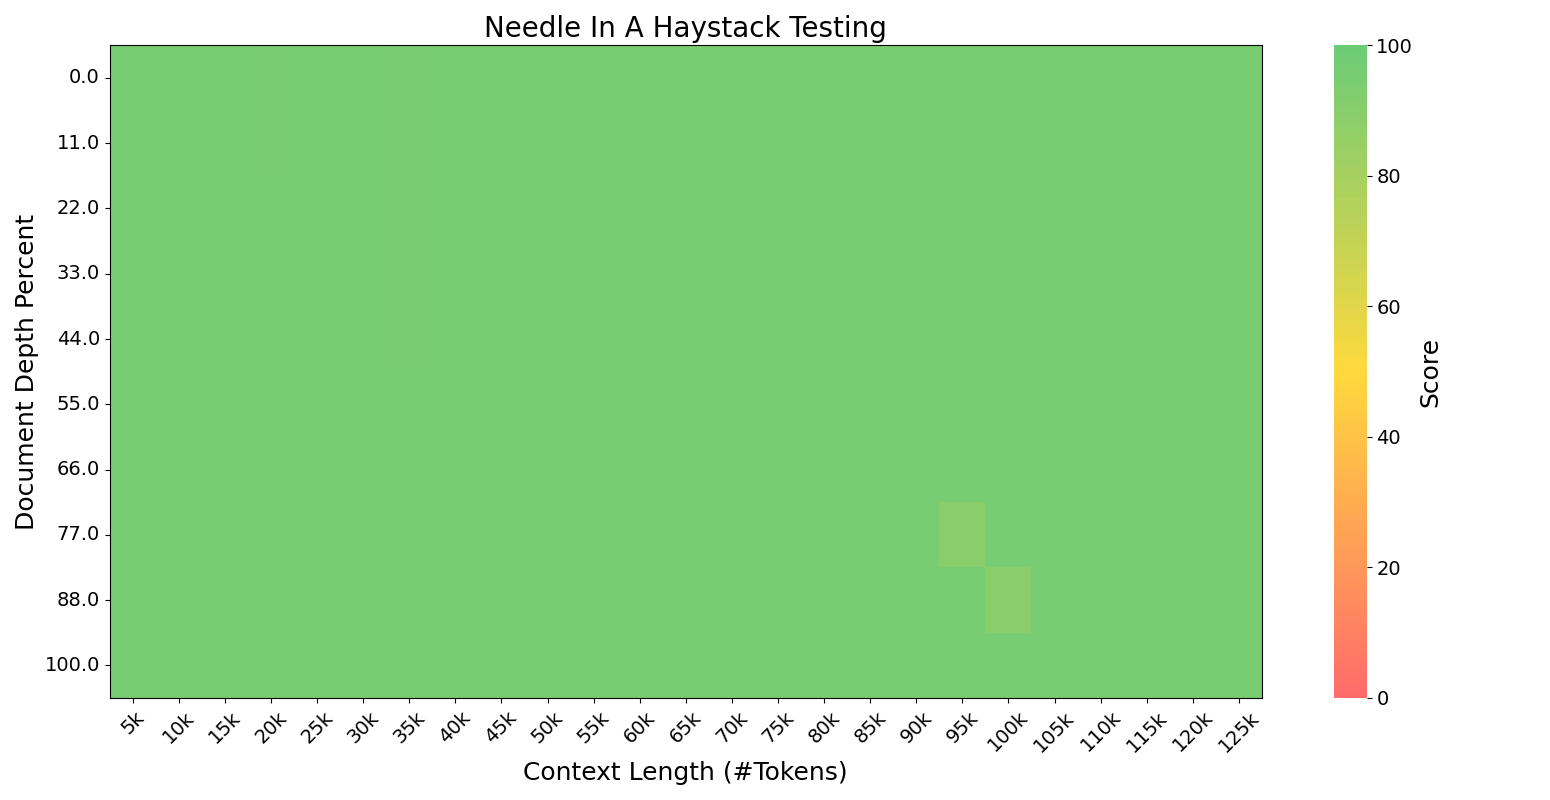
\includegraphics[width=0.7\textwidth]{figs/long_test.png}
    \caption{{Evaluation results on the ``Needle In A Haystack'' (NIAH) tests.} Following supervised fine-tuning, \texttt{Ling-mini-2.0} performs well across all context window lengths up to 128K.}
    \label{fig:long_test}
\end{figure*}




{\bfseries Reasoning Ability Pre-Activation.}
In the following 600B tokens of mid-training, we maintain a high proportion of reasoning data and introduce additional high-quality chain-of-thought (CoT) corpora. 
We continue training on this high-quality data at a higher learning rate and achieve robust performance by merging mid-training checkpoints. 
We find that the early introduction of CoT data during the latter pretraining phase effectively ``pre-activates'' the model's reasoning capabilities. 
This provides a higher ceiling for reasoning performance and a more stable foundation for subsequent fine-tuning and reinforcement learning stages. We further demonstrate the efficacy of this strategy in enhancing the model's reasoning abilities in Section~\ref{sec:eval_base_results}.



\subsubsection{WSM Scheduler}
\label{sec:merging}
Learning-rate (LR) decay has long been viewed as essential for effective LLM mid-training, but it restricts flexibility and increases tuning overhead. To enable a more flexible and effective process, the Ling 2.0 series adopts the novel WSM (warmup-stable-merge) scheduler~\citep{tian2025wsmdecayfreelearningrate}, which replaces LR decay with checkpoint merging and delivers superior performance. 

\paratitle{Theoretical Connection Between LR Decay and Checkpoint Merging. } 
We first establish the theoretical equivalence between checkpoint merging and LR decay. The merging process combines a sequence of checkpoints, $[\theta_n, \theta_{n+1}, \dots, \theta_{n+k}]$, into a single model, $\hat{\theta}_{n+k}$, via a weighted average. For analytical tractability, we assume the gradient updates between checkpoints are independent. By re-expressing each checkpoint $\theta_{n+j}$ in terms of a base checkpoint $\theta_n$ and the subsequent gradient updates ($g$), the derivation shows that the merging operation is mathematically equivalent to re-weighting the past gradients accumulated after the base checkpoint:
\begin{equation}
\label{eq:merge_as_gradient_reweighting}
    \hat{\theta}_{n+k} = \sum_{j=0}^{k} c_j \theta_{n+j} = \theta_n - \sum_{i=1}^{k} w_i g_{n+i-1}
\end{equation}
Here, the effective gradient weights, $w_i$, are determined by the original checkpoint merge weights, $c_j$. This equivalence demonstrates that checkpoint merging effectively simulates a post-hoc LR decay schedule, achieving an annealing effect without modifying the learning rate during the training phase itself.
Conversely, this relationship is invertible. Given a target LR decay schedule, represented by a desired sequence of monotonically non-increasing gradient decay coefficients $\{w_i\}_{i=1}^k$ (where $1 \ge w_1 \ge w_2 \ge \dots \ge w_k \ge 0$), we can uniquely determine the non-negative checkpoint weights $\{c_j\}_{j=0}^k$ that satisfy Equation~\ref{eq:merge_as_gradient_reweighting}:
\begin{equation}
\begin{cases}
    c_k = w_k \\
    c_j = w_j - w_{j+1}, & \text{for } j \in [1, k-1] \\
    c_0 = 1 - \sum_{j=1}^{k} c_j = 1 - w_1
\end{cases}
\label{eq:inverse_formula}
\end{equation}
This establishes a bidirectional conversion between LR decay and checkpoint merging, demonstrating that any LR decay schedule can be replicated through an appropriate merging strategy. 

\label{sec:main}
\begin{figure*}[t]
    \centering
    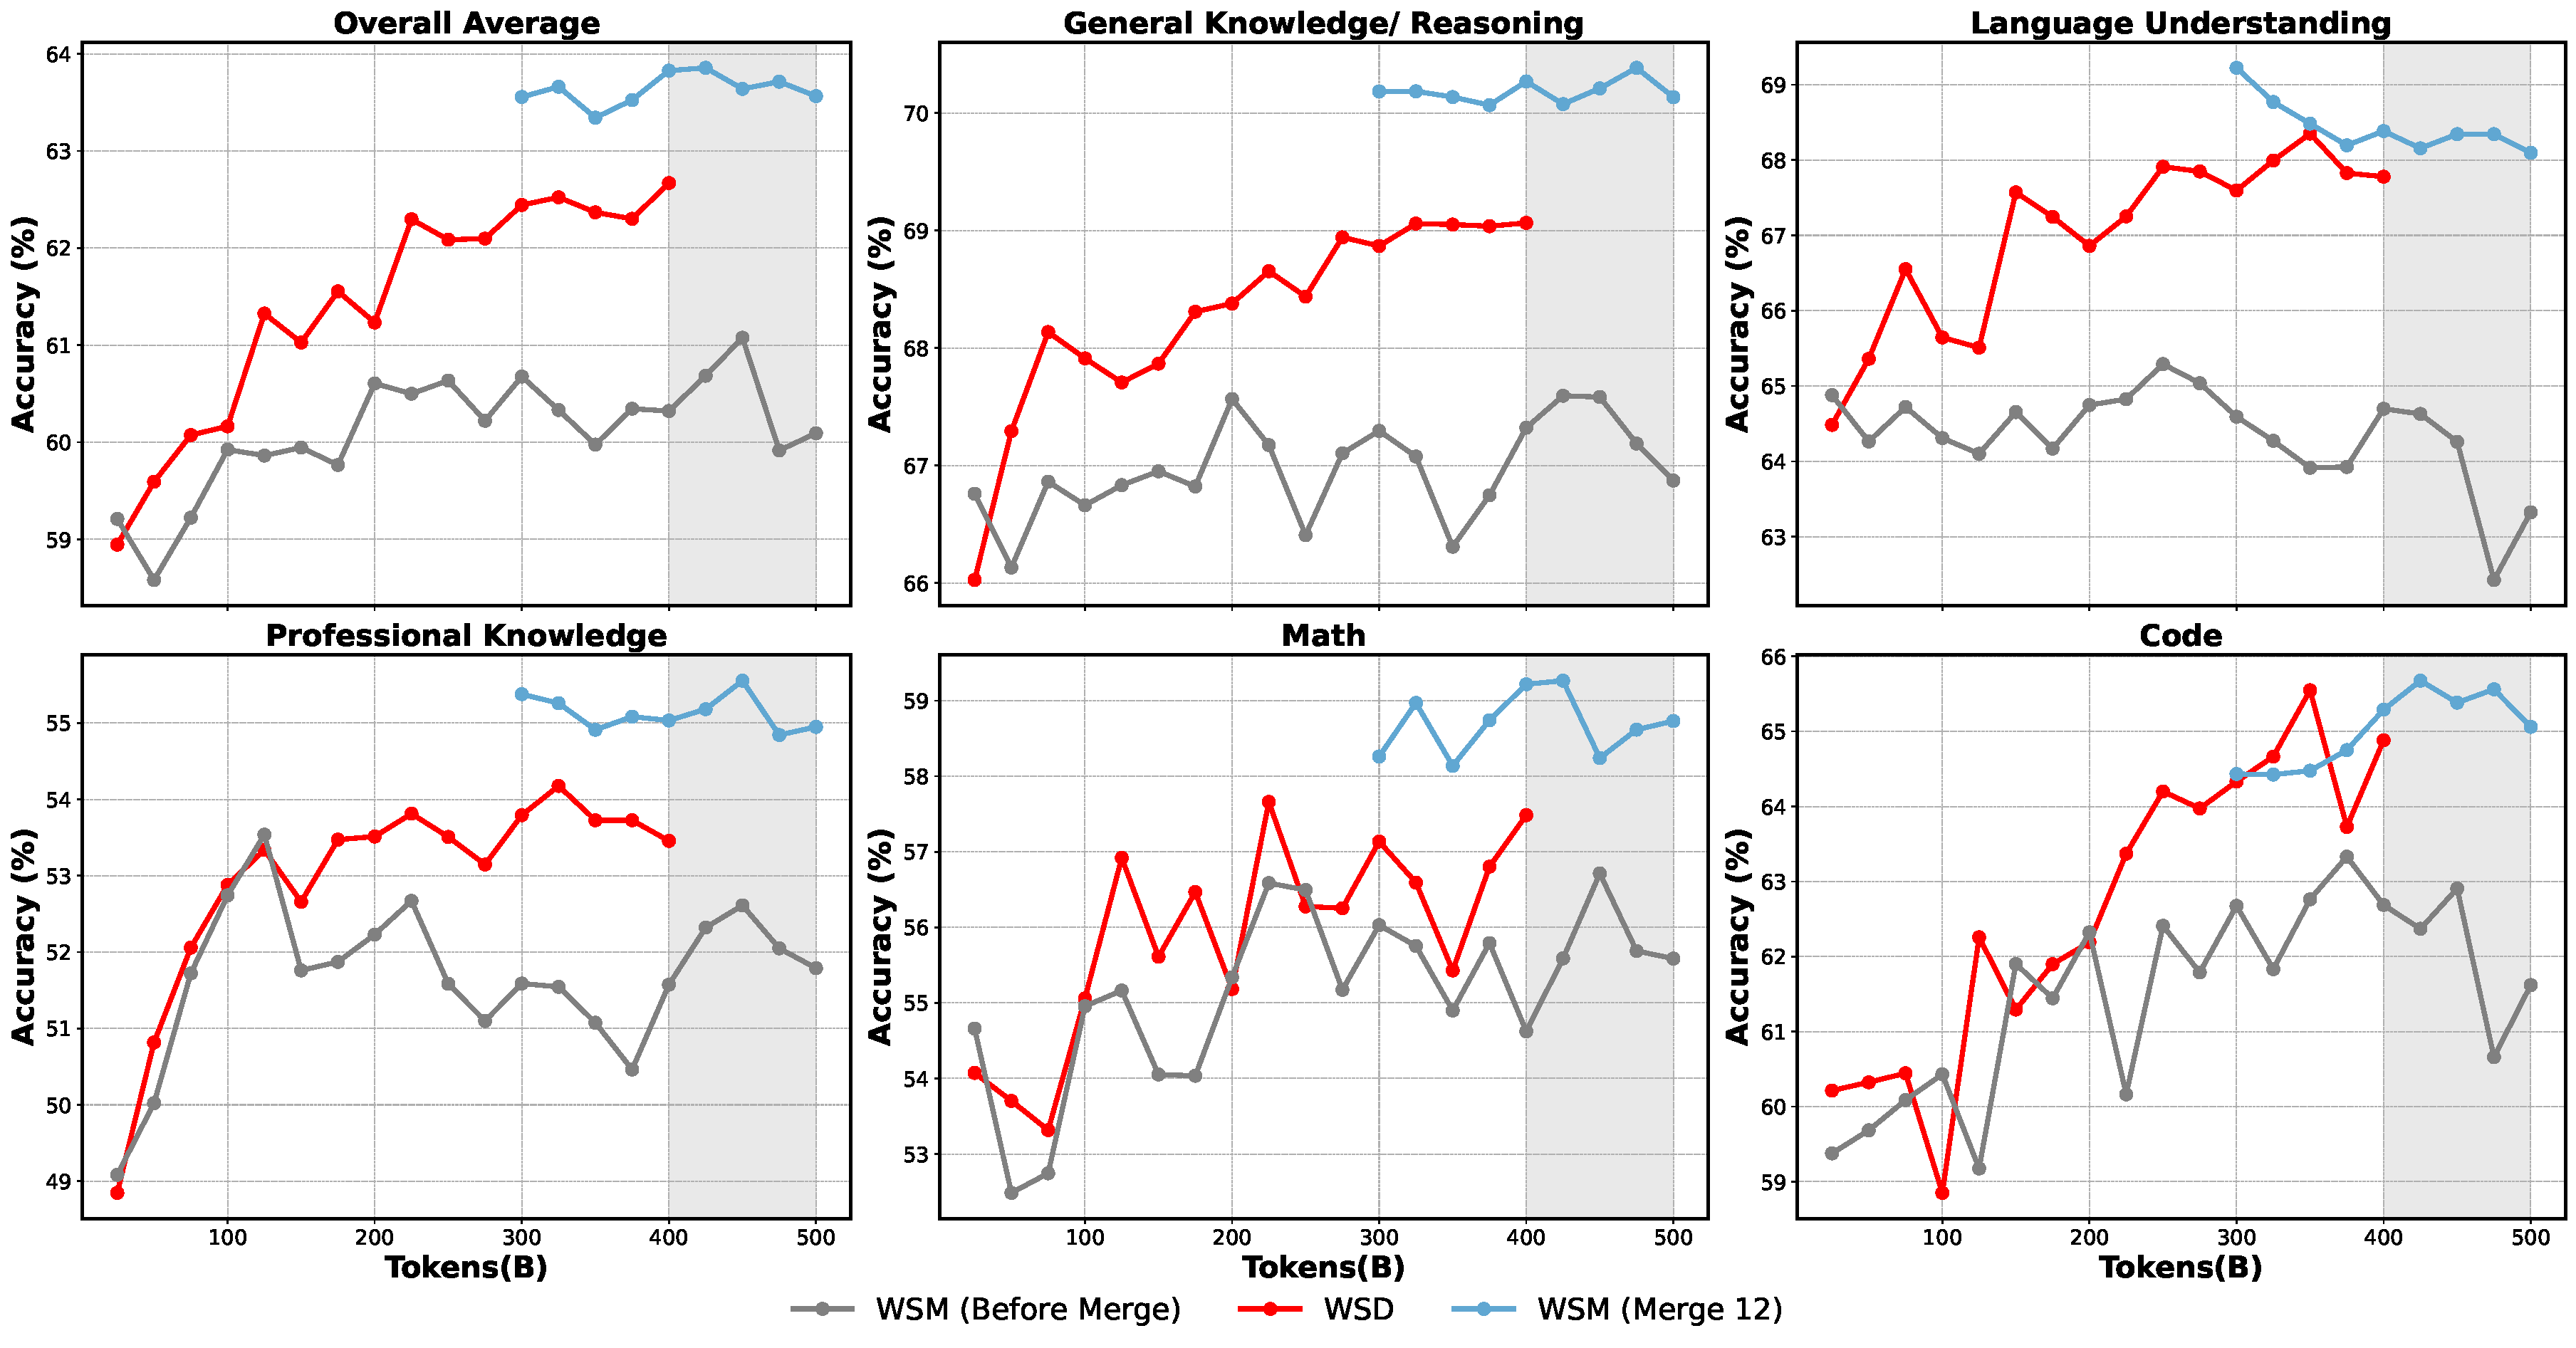
\includegraphics[width=0.85\textwidth]{figs/wsm.pdf}
    \caption{{Comprehensive performance comparison between our WSM scheduler (via checkpoint merging) and standard WSD scheduler (via LR decay).} Both approaches are initialized from the same pre-trained checkpoint. Notably, while WSD requires predetermined decay strategy (e.g., decay over 400B tokens in this study), WSM eliminates such constraints, enabling seamless training continuation (gray regions) and flexible decay behavior approximation.}
    \label{fig:wsm_vs_wsd}
\end{figure*}


\paratitle{Overall Performance and Heuristic Improvements. } 
A comprehensive comparison reveals that the proposed WSM scheduler consistently outperforms the strong WSD baseline~\citep{hu2024minicpm} across the majority of evaluated tasks (Figure~\ref{fig:wsm_vs_wsd}). Specifically, WSM yields an average improvement of +1 to +2 points on leaderboard scores across all benchmark categories. 
Crucially, WSM requires no prior choices about when to start LR decay or how long the decay phase should last (i.e., the decay data budget), offering greater flexibility and scalability than WSD. Moreover, it produces models with more balanced capability profiles.
To validate robustness, we further applied supervised fine-tuning for 5 epochs on checkpoints from both schedulers under identical settings, confirming that WSM's advantage persists beyond post-training.
As a practical heuristic to further improve stability, we select the top-$N$ checkpoints in the final stage of mid-training based on validation performance and average their parameters. For the final {Ling 2.0} model, we set $N=32$.


\subsection{Pre-training Evaluation}
To evaluate the pre-training of Ling 2.0, we focus on both the final model’s benchmark performance and the performance dynamics throughout pretraining. 

\subsubsection{Evaluation of Pre-training Dynamics}

{\bfseries Selecting and Adapting Benchmarks for Pre-training. }
During pre-training, base models often exhibit limited instruction-following ability, which can lead to misleading evaluations. To mitigate this, we propose a framework for selecting and adapting benchmarks. Specifically, we score candidate benchmarks by (i) their stability over  the course of training and (ii) their consistency with post-training performance, quantified via Kendall’s rank correlation. Only benchmarks that satisfy both criteria are retained to monitor the base model throughout training. 
For benchmarks that fail to meet these criteria, we adapt them to improve stability via in-context, light-instruction prompts or fill-in-the-blank formats~\citep{luan2025bose}.

{\bfseries Optimizing Evaluation Methods During Pre-training. }
Beyond benchmark design, the evaluation process itself can suffer from instability. We systematically diagnose this instability, attributing it to two distinct sources: parameter instability, arising from training stochasticity, and evaluation instability, caused by noisy measurement protocols. 
To counteract these issues, we employ a two-pronged approach~\citep{wang2025map}. First, we use checkpoint merging to mitigate parameter instability by averaging the weights of recent checkpoints, thereby smoothing the model's trajectory in the parameter space. Second, we adopt the Pass@k metric to address evaluation instability, as it offers a more robust, low-variance statistical estimate of a base model's true capability. Extensive experiments demonstrate that this combined approach yields significantly smoother performance curves, providing a more reliable and faithful lens for observing training dynamics.

\subsubsection{{Evaluation of Ling 2.0 Base Models}}
\label{sec:eval_base_results}

{\bfseries Benchmarks and Configurations.} 
The suite spans mathematics, coding, reasoning, knowledge, and multilingual ability. Unless noted, we report EM/Acc or Pass@1 with standardized prompting and decontamination. The evaluation datasets for pre-trained base models includes 33 benchmarks, which are categorized as follows:
\begin{itemize}
    \item \textbf{Math Tasks}: CMath~\citep{cmath} (3-shot, CoT), 
    MATH~\citep{math} (0-shot, CoT), 
    CollegeMath~\citep{college-math} (4-shot, CoT), 
    MinervaMath~\citep{Minerva} (4-shot, CoT), 
    FinanceReasoning~\citep{finance-reasoning} (3-shot, CoT), 
    OlympiadBench~\citep{olympiadbench} (3-shot, CoT), 
    TheoremQA~\citep{theoremqa} (5-shot), 
    OmniMath~\citep{omni-math} (3-shot, CoT), 
    AIME25~\citep{aime25} (0-shot, CoT).

    \item \textbf{Coding Tasks}: HumanEval~\citep{humaneval} (0-shot), 
    HumanEval-cn~\citep{humaneval_cn} (0-shot), 
    HumanEval-Plus~\citep{mbpp+} (0-shot), 
    CruxEval~\citep{cruxeval} (1-shot, CoT), 
    MultiPL-E~\citep{multipl-e} (0-shot), 
    LiveCodeBench\footnote{LiveCodeBench contains 454 problems released between Aug 2024 and May 2025. }~\citep{livecodebench} (0-shot), 
    BigCodeBench~\citep{bigcodebench} (0-shot), 
    BIRD-SQL~\citep{birdsql} (0-shot), 
    CodeCriticBench~\citep{codecriticbench} (2-shot), 
    CodeForces~\citep{codeforces} (0-shot, CoT).

    \item \textbf{General Reasoning Tasks}: 
    CommonSenseQA~\citep{talmor2018commonsenseqa} (5-shot), 
    WorldSense~\citep{worldsense} (0-shot), 
    Multi-LogiEval~\citep{Multilogieval} (2-shot, CoT), 
    AutoLogi~\citep{autologi} (3-shot, CoT), 
    ProntoQA~\citep{PrOntoQA} (1-shot, CoT). 

    \item \textbf{Knowledge Tasks}: ARC~\citep{arc} (0-shot), 
    MMLU~\citep{mmlu} (5-shot), 
    MMLU-Pro~\citep{mmlu-pro} (5-shot), 
    C-Eval~\citep{ceval} (5-shot), 
    CMMLU~\citep{cmmlu} (5-shot).

    \item \textbf{Multilingual Tasks}: 
    MMMLU\footnote{MMMLU language coverage may differ across baselines.}~\citep{mmmlu} (0-shot), 
    mARC~\citep{marc} (0-shot), 
    MultiGSM~\citep{mgsm} (4-shot, CoT), 
    HumanEvalXL~\citep{humanevalxl} (0-shot).
\end{itemize}
We compare Ling 2.0 base models against the base models of Qwen2.5~\citep{qwen2.5} and Qwen3~\citep{qwen3} series, as well as other leading open-source models, including Hunyuan-7B~\citep{hunyuan-7b}, Seed-OSS-36B~\citep{seed2025seed-oss}, DeepSeek-V3.1~\citep{deepseekai2024deepseekv3technicalreport} and Kimi-K2~\citep{kimiK2}.

{\bfseries Evaluation Results.} 
Table~\ref{tab:mini-base-benchmarks},~\ref{tab:flash-base-benchmarks} and~\ref{tab:ling-1T-base-benchmarks} present the evaluation results for the Ling 2.0 base models. All models are evaluated using our unified internal evaluation framework to ensure a fair and consistent comparison. 
As introduced in Section~\ref{sec:mid-training}, we specifically compare model versions with and without the integration of high-quality Chain-of-Thought (CoT) data to demonstrate the efficacy of this strategy. The key findings are as follows: 
\begin{itemize}
    \item \textbf{Verified 7× Efficiency Leverage}: 
    Both our \texttt{Ling-mini-2.0-base}, \texttt{Ling-flash-2.0-base}, and \texttt{Ling-1T-base} achieve performance comparable or superior to other state-of-the-art open-source models of similar scale. 
    In particular, \texttt{Ling-mini-2.0-base} and \texttt{Ling-flash-2.0-base} achieve overall performance comparable to the dense Qwen3 8B base and Seed-OSS-36B base, while using less than one-seventh of their non-embedding activated parameters, confirming the 7× efficiency leverage claimed at the outset of Ling 2.0.
    
    \item \textbf{Exceptional Math and Code Capabilities}: 
    Notably, the Ling 2.0 series exhibits a significant advantage in mathematics and coding tasks, indicating strong capabilities in structured reasoning, algorithmic thinking, and programming. For example, \texttt{Ling-1T} achieves superior results on benchmarks such as MathBench, CollegeMath, MinervaMath, OmniMath, HumanEval-Plus, CruxEval, MultiPL-E, etc. 
    \item \textbf{Effective Reasoning Pre-activation via CoT Data}: 
    Integrating high-quality CoT data during mid-training effectively ``pre-activates'' the models' reasoning abilities. This leads to substantial gains on reasoning-intensive benchmarks like MATH, AIME and LiveCodeBench, while maintaining performance on other benchmarks. Crucially, this pre-activated advantage persists through subsequent SFT and RL phases (as shown in Figure~\ref{fig:apexeval}), significantly enhancing their effectiveness.
\end{itemize}


\begin{table*}[h]
\centering
\caption{{Comparison among \texttt{Ling-mini-2.0-base} and other representative open-source base models. }}
\label{tab:mini-base-benchmarks}
\small
{
\begin{tabular}{lcccc}
\toprule
\textbf{Benchmark} & \textbf{\splitcell{Hunyuan-7B \\ Base}}  & 
\textbf{\splitcell{Qwen3-8B \\ Base}}  & \textbf{\splitcell{\texttt{Ling-mini-2.0} \\ Base \\ w/o CoT Data}} & \textbf{\splitcell{\texttt{Ling-mini-2.0} \\ Base \\ w/ CoT Data}} \\
\midrule
\multicolumn{5}{c}{\textit{Math}} \\
\midrule
CMath (Acc.) & \underline{92.26} & 88.16 & \textbf{92.81} & 92.08\\
MathBench (Acc.) & 73.19 & 74.21 & \underline{76.01} & \textbf{76.06} \\
CollegeMath (Acc.) & \underline{70.62} & 66.00 & 69.84 & \textbf{72.50}\\
OlympiadBench (Acc.) & 20.44 & 22.22 & \underline{23.85} & \textbf{24.30}\\
TheoremQA (Acc.) & 31.00 & 35.00 & \underline{37.25} & \textbf{39.00}\\
OmniMath (Acc.) & 20.10 & 20.20 & \textbf{24.40} & \underline{24.20}\\
MATH (Acc.) & 65.10 & \underline{76.98} & 61.96 & \textbf{82.52}\\
AIME25 (Pass@1) & \underline{14.79} & 13.54 & 2.08 & \textbf{43.75} \\
\midrule
\multicolumn{5}{c}{\textit{Code}} \\
\midrule
HumanEval (Pass@1) & 64.02 & \textbf{84.76} & 81.71 & \underline{83.54} \\
HumanEval-cn (Pass@1) & 72.56 & \underline{73.78} & 73.17 & \textbf{77.44} \\
HumanEval-Plus (Pass@1) & 51.22 & \underline{75.61} & \underline{75.61} & \textbf{76.22}\\
CruxEval (Pass@1) & \underline{63.69} & 61.56 & 60.56 & \textbf{66.44} \\
MultiPL-E (Pass@1) & 54.97 & 57.58 & \underline{65.31} & \textbf{65.94}\\

BigCodeBench (Pass@1) & 41.67 & 40.70 & \textbf{44.30} & \underline{43.68} \\
BIRD-SQL (Acc.) & 22.75 & 13.07 & \textbf{26.17} & \underline{26.08} \\
CodeForces (Pass@1) & 26.91 & 18.22 & \textbf{47.18} & \underline{42.50} \\

LiveCodeBench (Pass@1) & \underline{20.15} & 14.10 & 13.71 & \textbf{34.47}\\
\midrule
\multicolumn{5}{c}{\textit{General Reasoning}} \\
\midrule
CommonSenseQA (EM) & 80.59 & \textbf{83.78} & 80.18 & \underline{81.08} \\

WorldSense (EM) & \textbf{59.39} & 57.83 & 57.61 & \underline{59.09} \\
ProntoQA (EM) & 72.50 & \underline{79.00} & 76.00 & \textbf{81.00} \\
\midrule
\multicolumn{5}{c}{\textit{Knowledge}} \\
\midrule
ARC-e (EM) & 96.47 & \underline{97.00} & \textbf{97.35} & \underline{97.00} \\
ARC-c (EM) & 89.49 & \textbf{91.86} & 90.17 & \underline{90.51} \\
MMLU (EM) & \textbf{79.95} & \underline{78.62} & 74.21 & 74.26\\
MMLU-Pro (EM) & \textbf{61.22} & \underline{50.83} & 47.36 & 47.70\\
C-Eval (EM) & \textbf{83.90} & 83.19 & \underline{83.57} & 80.41\\
CMMLU (EM) & \textbf{82.22} & \underline{81.31} & 81.29 & 79.98\\
\midrule
\multicolumn{5}{c}{\textit{Multilingual}} \\
\midrule
mARC (EM) & 48.34 & \textbf{80.70} & 64.46 & \underline{65.33} \\
MMMLU (EM) & 42.36  & \textbf{60.02} & \underline{51.28} & 50.14\\
MultiGSM (Acc.) & 53.67 & \textbf{77.60} & 66.6 0& \underline{67.87} \\
HumanEvalXL (Pass@1) & 58.59 & \textbf{69.53} & \underline{68.28}	& 65.31 \\
\bottomrule
\end{tabular}
}
\end{table*}

\begin{table*}[h]
\centering
\caption{{Comparison among \texttt{Ling-flash-2.0-base} and other representative open-source base models. }}
\label{tab:flash-base-benchmarks}
\small
{
\begin{tabular}{lcccc}
\toprule
\textbf{Benchmark} & \textbf{\splitcell{Qwen2.5-72B \\ Base}}  & 
\textbf{\splitcell{Seed-OSS-36B \\ Base}} & \textbf{\splitcell{\texttt{Ling-flash-2.0} \\ Base \\ w/o CoT Data}} & 
\textbf{\splitcell{\texttt{Ling-flash-2.0} \\ Base \\ w/ CoT Data}}\\
\midrule
\multicolumn{5}{c}{\textit{Math}} \\
\midrule
MathBench (Acc.) & 76.65 & \underline{79.70} & \textbf{80.18} & 77.69 \\
FinanceReasoning (Acc.) & 74.60 & \underline{74.98} & 74.43 & \textbf{76.44} \\
TheoremQA (Acc.) & 39.00 & \underline{44.25} & \textbf{46.25} & 43.50\\
OmniMath (Acc.) & 18.40 & 20.40 & \underline{27.30} & \textbf{28.30}\\
MATH & 76.46 & \textbf{88.64} & 66.26 & \underline{79.54}\\
\midrule
\multicolumn{5}{c}{\textit{Code}} \\
\midrule
HumanEval (Pass@1) & 82.32 & 85.37 & \underline{89.02} & \textbf{89.63} \\
HumanEval-cn (Pass@1) & 78.66 & 80.49 & \textbf{84.15} & \underline{82.32} \\
HumanEval-Plus (Pass@1) & 73.78 & 78.66 & \underline{81.10} & \textbf{83.54}\\
CruxEval (Pass@1) & 63.10 & \underline{73.12} & 69.50 & \textbf{77.38}\\
MultiPL-E (Pass@1) & 60.00 & 67.04 & \underline{69.33} &\textbf{69.70}\\

BigCodeBench (Pass@1) & 41.18 & \textbf{52.89} & 50.88 & \underline{52.37} \\
CodeCriticBench (Acc.) & 67.94 & 65.12 & \underline{70.40} & \textbf{70.93} \\
CodeForces (Pass@1) & 17.81 & 19.57 & \underline{36.86} & \textbf{47.54} \\

\midrule
\multicolumn{5}{c}{\textit{General Reasoning}} \\
\midrule
CommonSenseQA (EM) & \textbf{88.12} & 75.02 & 86.73 & \underline{87.71} \\
Multi-LogiEval (EM) & 74.23 & \textbf{81.72} & \underline{75.51} & 74.67 \\
AutoLogi (Acc.) & 58.29 & 57.36 & \underline{58.54} & \textbf{61.10}\\
\midrule
\multicolumn{5}{c}{\textit{Knowledge}} \\
\midrule
ARC-e (EM) & \underline{98.06} & \underline{98.06} & 97.53 & \textbf{98.24}\\
ARC-c (EM) & \textbf{96.27} & 94.58 & 95.59 & \underline{95.93} \\
MMLU (EM) & \textbf{86.29} & \underline{84.99} & 82.67 & 82.98\\
MMLU-Pro (EM) & \textbf{61.41} & 60.64 & 59.43 & \underline{60.73}\\
C-Eval (EM) & 88.14 & 88.59 & \underline{88.64} & \textbf{89.06}\\
CMMLU (EM) & \textbf{89.56} & 87.07 & 87.41 & \underline{87.90} \\
\midrule
\multicolumn{5}{c}{\textit{Multilingual}} \\
\midrule
MMMLU (EM) & \textbf{72.70} & \underline{70.57} & 63.83 & 62.76\\
mARC (EM) & \textbf{88.84} & \underline{85.21} & 81.87 & 82.07 \\
MultiGSM (Acc.) & \underline{82.87} & \textbf{85.2} & 80.33 & 80.07 \\
HumanEvalXL (Pass@1) & \textbf{76.25} & 73.12 & \underline{75.78} & 71.88 \\
\bottomrule
\end{tabular}}
\end{table*}


\begin{table*}[h]
\centering
\caption{{Comparison among \texttt{Ling-1T-base} and other representative open-source base models. }}
\label{tab:ling-1T-base-benchmarks}
\small
{
\begin{tabular}{lcccccc}
\toprule
\textbf{Benchmark} & \textbf{\splitcell{DeepSeek-V3.1 \\ Base}}  & \textbf{\splitcell{Kimi-K2 \\ Base}}  &  \textbf{\splitcell{\texttt{Ling-1T} \\ Base \\ w/o CoT Data}} & \textbf{\splitcell{\texttt{Ling-1T} \\ Base \\ w/ CoT Data}}\\
\midrule
\multicolumn{5}{c}{\textit{Math}} \\
\midrule

MathBench (Acc.) & 73.30 & 80.26 & \underline{81.27} & \textbf{82.11} \\
CollegeMath (Acc.) & 63.88 & 70.69 & \underline{75.02} & \textbf{75.48}\\
MinervaMath (Acc.) & 48.90 & \underline{55.88} & 50.00 & \textbf{62.87}\\

TheoremQA (Acc.) & 43.75 & \textbf{47.50} & 44.88 & \underline{46.62}\\
OmniMath (Acc.) & 21.10 & 29.90 & \textbf{35.70} & \underline{33.60}\\

MATH (Acc.) & 35.64 & \underline{76.40} & 67.42 & \textbf{82.78}\\
\midrule
\multicolumn{5}{c}{\textit{Code}} \\
\midrule
HumanEval (Pass@1) & \underline{74.39} & \textbf{89.63} & \textbf{89.63} & \textbf{89.63} \\
HumanEval-cn (Pass@1) & 72.56 & \textbf{85.37} & \underline{84.76} & \textbf{85.37} \\
HumanEval-Plus (Pass@1) & 65.85 & \textbf{84.15} & \textbf{84.15} & \underline{83.54}\\
CruxEval (Pass@1) & 69.81 & \underline{78.25} & 74.88 & \textbf{80.88}\\
MultiPL-E (Pass@1) & 59.50 & 64.15 & \textbf{70.70} & \underline{69.94}\\
CodeCriticBench (Acc.) & 67.72 & \underline{70.88} & \textbf{71.56} & 66.09 \\
CodeForces (Pass@1) & 45.64 & 24.79 & \underline{55.32} & \textbf{55.78} \\

\midrule
\multicolumn{5}{c}{\textit{General Reasoning}} \\
\midrule
CommonSenseQA (EM) & 85.83 & 85.42 & \underline{89.60} & \textbf{89.76} \\
WorldSense (EM) & 57.73 & 64.02 & \textbf{67.43} & \underline{66.99}\\
AutoLogi (Acc.) & 63.02 & \underline{63.60} & 63.21 & \textbf{65.76}\\
\midrule
\multicolumn{5}{c}{\textit{Knowledge}} \\
\midrule
ARC-e (EM) & 97.18 & \textbf{98.77} & 97.71 & \underline{98.59} \\
ARC-c (EM) & 92.88 & 95.59 & \underline{96.61} & \textbf{97.63} \\
MMLU (EM) & \textbf{88.44} & \underline{88.32} & 85.91 & 86.03\\
MMLU-Pro (EM) & \underline{67.75} & 67.50 & 66.70 & \textbf{67.91}\\
C-Eval (EM) & 90.67 & \textbf{91.72} & \underline{91.41} & 90.75\\
CMMLU (EM) & 88.19 & \textbf{90.35} & 90.18 & \underline{90.26}\\
\midrule
\multicolumn{5}{c}{\textit{Multilingual}} \\
\midrule
MMMLU (EM) & 69.46 & \textbf{72.91} & \underline{70.13} & 68.68\\
mARC (EM) & 83.62 & \textbf{88.40} & 86.64 & \underline{86.68} \\
MultiGSM (Acc.) & 82.20 & \textbf{86.87} & 81.87 & \underline{85.40} \\
HumanEvalXL (Pass@1) & 75.00 & \underline{80.94} & \textbf{81.72} & 80.62 \\
\bottomrule
\end{tabular}}
\end{table*}




